\chapter{Experiment}\label{ch.exp}

Having now established what results we expect to find in an experiment, we must perform an actual experiment to have something with which to compare our expectations. 

As was perhaps already given away by the title, this thesis will use the \textsc{atlas}\footnote{\textbf{A} \textbf{T}oroidal \textbf{L}HC \textbf{A}pparatu\textbf{s}.} experiment, which is part of the Large Hadron Collider complex at \textsc{cern}\footnote{\textbf{C}onseil \textbf{E}uropéen pour la \textbf{R}echerche \textbf{N}ucléaire. When the council tasked with creating the european nuclear research laboratory became the organisation tasked with running that laboratory, its name changed to Organisation Européenne pour la Recherche Nucléaire---the European Organisation for Nuclear Research, but the acronym stayed the same. Acronyms, it seems, are not only ubiquitous, but also immutable.} in Geneva.

\section{The Large Hadron Collider}

The purpose of the Large Hadron Collider is to accelerate protons\footnote{Or heavy ions, on the occations when the LHC runs heavy ion collision experiments.} (which are a species of hadrons) to very high kinetic energies, and then bringing them to collide with other protons, which have similarly been accelerated to very high energies. As a necessity dictated by have gone to these very high energies, the accelerator is also quite large.

\begin{figure}[htp]
\begin{center}
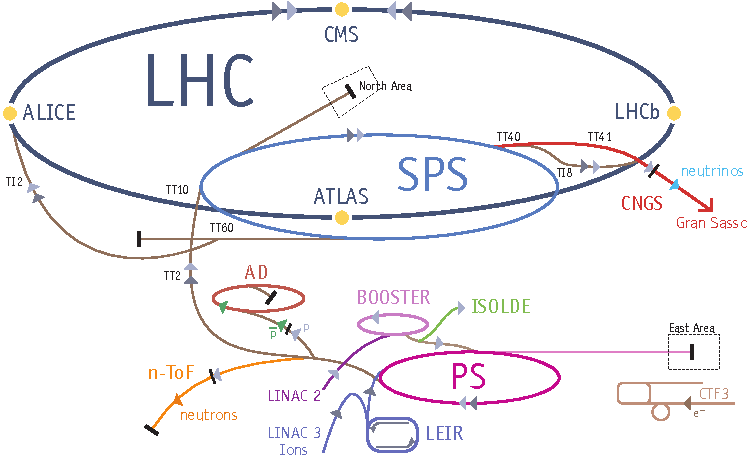
\includegraphics[width=.8\textwidth]{Cernrings}
\end{center}
\begin{minipage}[b]{\textwidth}
\caption{A schematic view of the \textsc{cern} accelerator complex \cite{cernbro}, which accelerates the protons or ions used in collision experiments through several accelerators to progressively higher energies. The paths protons can take through the machine are marked with light gray triangles. The dark gray triangles mark the paths taken by lead ions when the Collider runs proton--lead or lead--lead collision experiments. Protons are `created' by ionising hydrogen atoms and then injected by \textcolor{Purple}{LINAC 2} into the \textcolor{Plum}{Booster ring}. From there, protons are accelerated by the Proton Synchrotron (\textcolor{Magenta}{PS}) and then the Super Protron Synchrotron (\textcolor{RoyalBlue}{SPS}) before finally being sent into the \textcolor{MidnightBlue}{LHC} ring. The LHC ring is the largest one, measuring approximately 27~km in circumference.}
\label{cernrings}
\end{minipage}
\end{figure}

The protons are accelerated to the appropriate energies by electric fields in radiofrequency cavities. They are then kept confined within the two beam pipes in the LHC ring---one for each of the two beams moving in either direction---by superconducting multipole magnets. The LHC does not, however, accelerate protons all the way from rest to its collision energy. It is the last part of a multi-stage machine, which is shown in schematic form in fig.~\ref{cernrings}. As an interesting aside, two of the intermediate stages in this machine, the Proton Synchrotron and the Super Proton Synchrotron were at one point \textsc{cern}'s main accelerator.

At the LHC, the beam energy was intended to be 7 TeV per beam, however several accidents when the machine was started has forced us to lower out ambitions for the time being. In 2012, when the data that will be used in this thesis was taken, the LHC ran at 4 TeV per beam, for a total collision energy of 8 TeV.

The two beam pipes cross another at four points around the LHC ring, the centres of the four detectors.

\section{The ATLAS detector}
The \textsc{atlas} detector sits at one of these interaction points, and is, along with CMS\footnote{The \textbf{C}ompact \textbf{M}uon \textbf{S}olenoid.}, a general purpose detector, designed to capture as much information as possible about collision events. To that end, the \textsc{atlas} detector uses three distinct types of detectors, arranged in concentric layers around the interaction point. From innermost to outermost, these are: the tracking system, the calorimeter system and the muon tracking system. The layout of the detector is shown in figure~\ref{allatlas}. For a more detailed description, see \cite{detectorpaper}.

\begin{figure}[htp]
\begin{minipage}[b]{.69\textwidth}
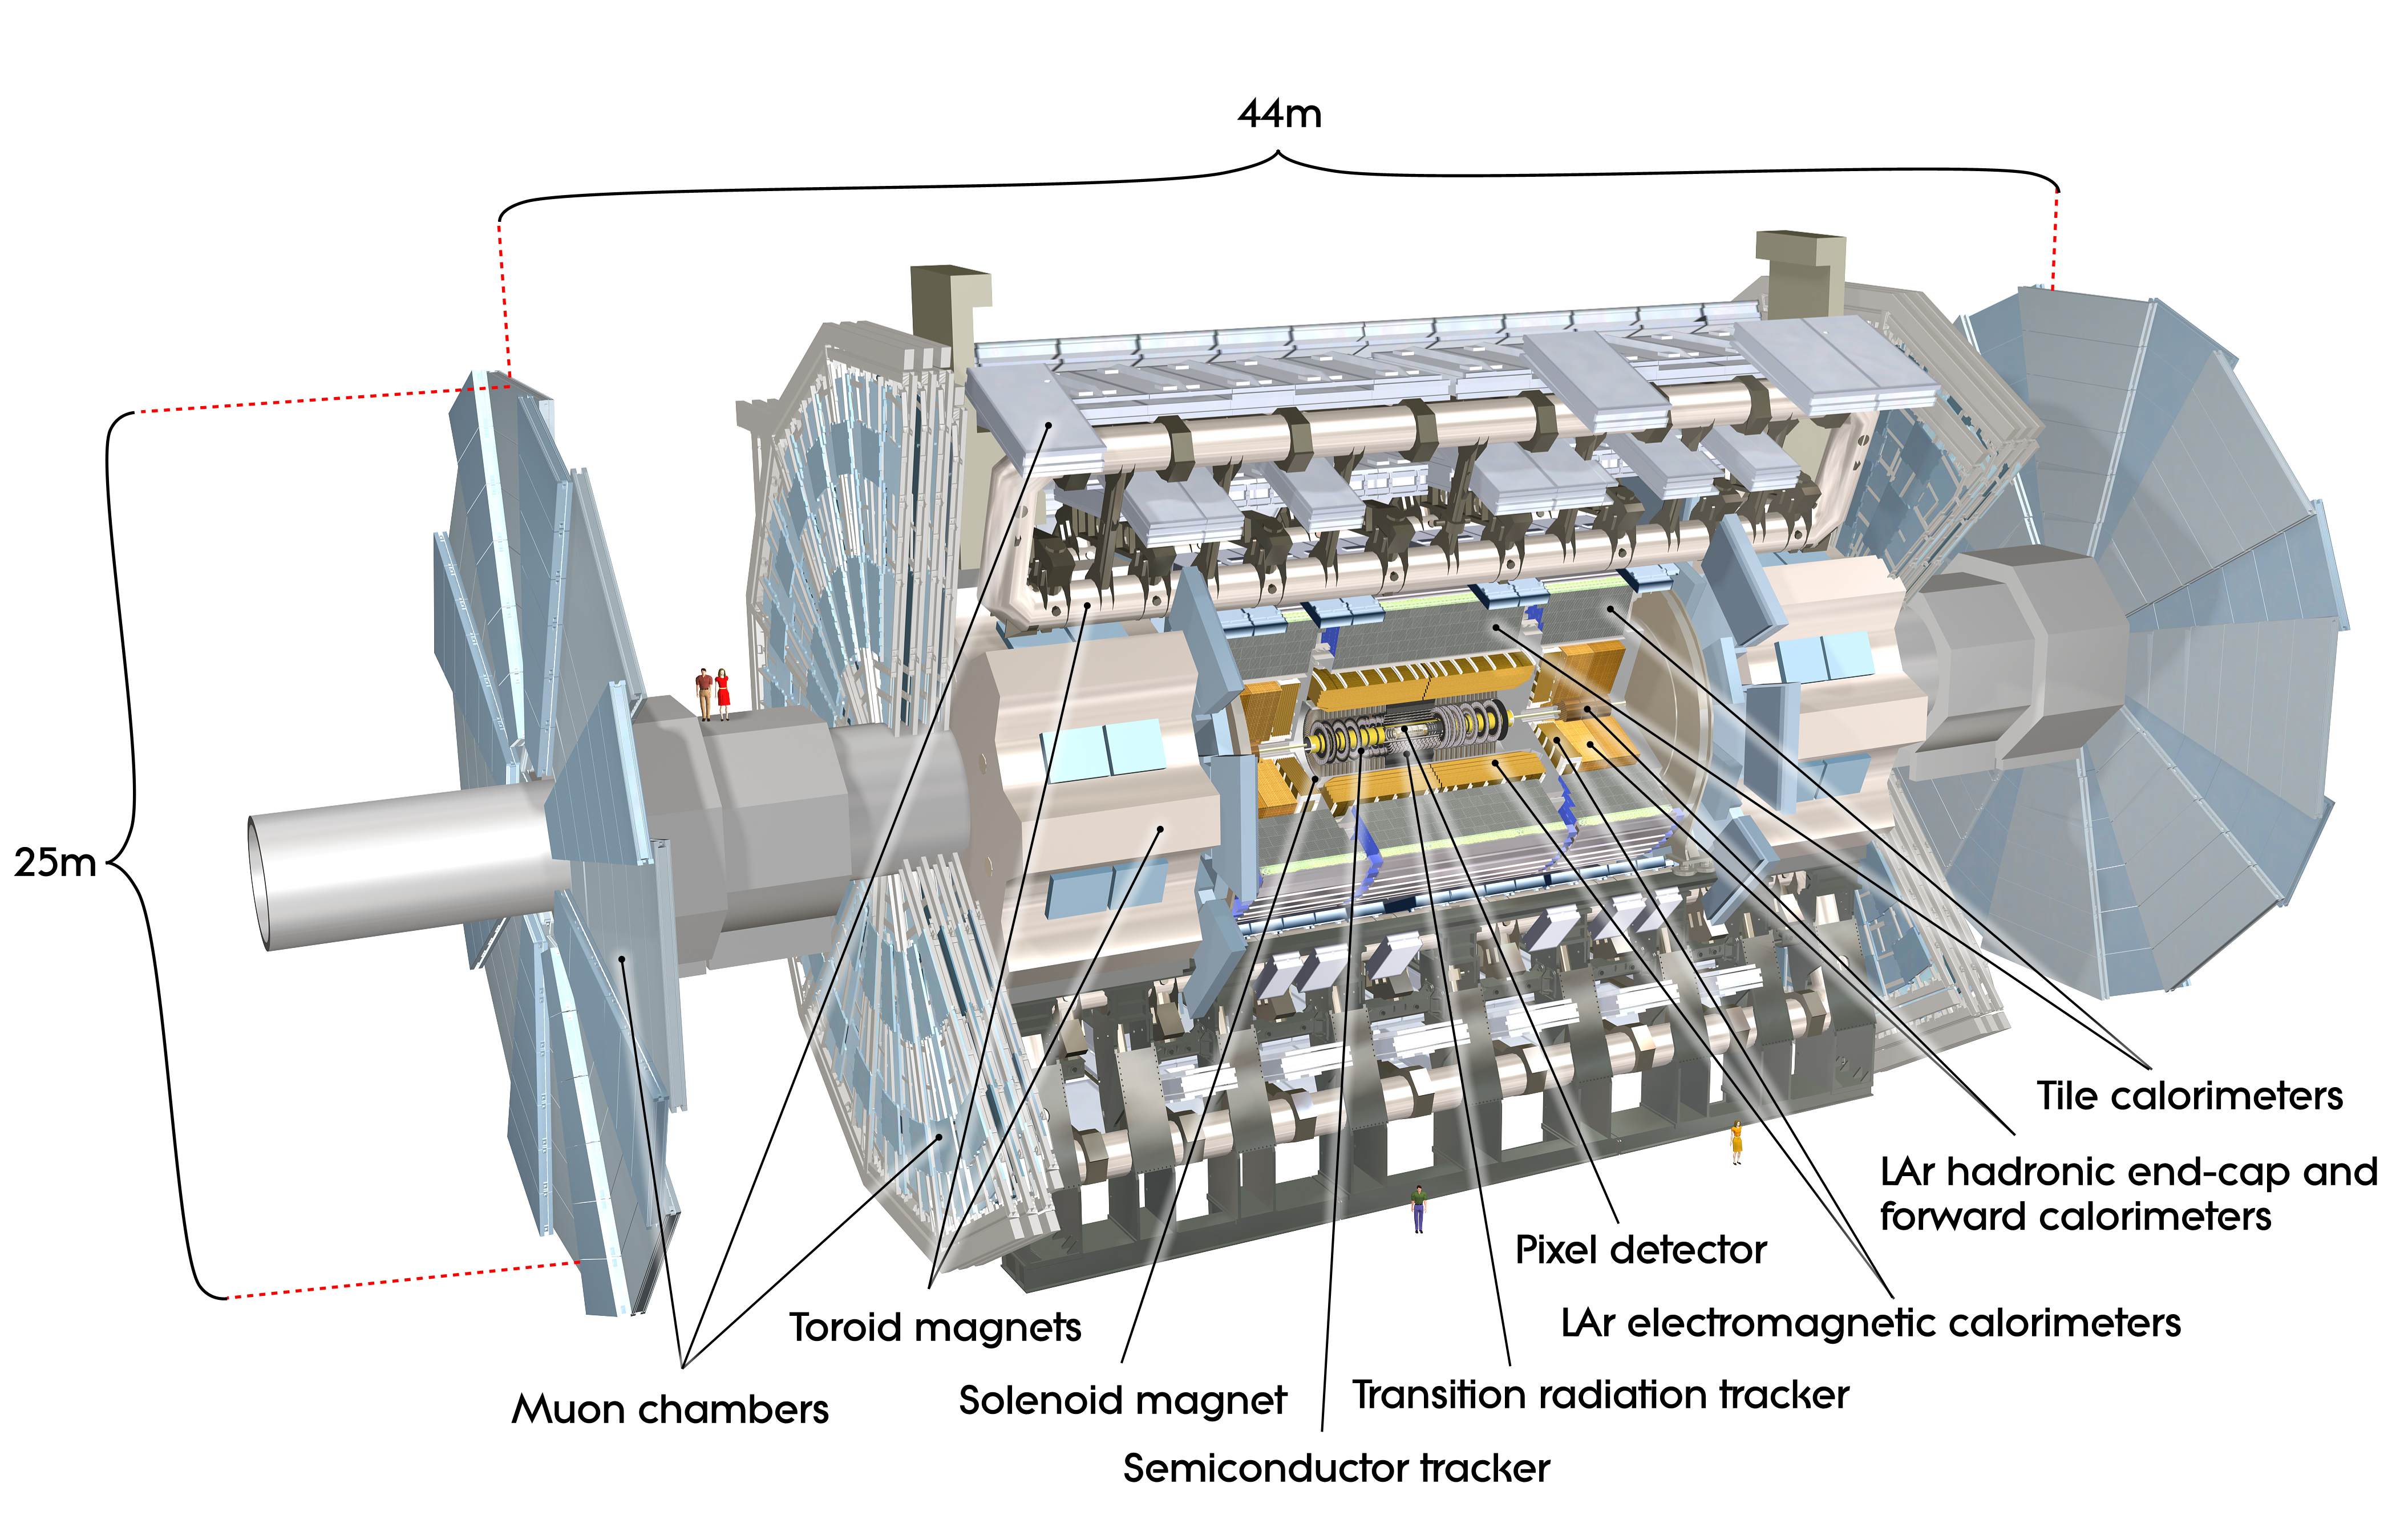
\includegraphics[width=1\textwidth]{AllAtlasBig}
\end{minipage}
\begin{minipage}[b]{.3\textwidth}
\caption{A diagram of the entire \textsc{atlas} detector \cite{atlasweb}. The overall structure is of a layered cylinder centred on the interaction point. We refer to those parts of the detector that make up the wall of the cylinder as the barrel section, and to the ends of the cylinder as the endcap. The electromagnetic calorimeter, which is the detector element that we will make the most use of here, is coloured orange in this drawing.}
\end{minipage}
\label{allatlas}
\end{figure}

\textsc{Atlas} defines its own coordinate system, centred on the interaction point, where the position in the angular direction, perpendicular to the beam pipe, is measured by the azimuthal coordinate $\phi$, and the angle to the beam pipe is measured in pseudorapidity $\eta$, which is defined as
\(\eta=-\ln[\tan(\theta/2)],\)
where $\theta$ is the polar angle to the beam pipe in radians \cite{green:eta}. The pseudorapidity $\eta$ is a simple transformation of $\theta$---it is 0 at $\theta=\pi/2$, $\infty$ at $\theta=0$ and $-\infty$ at $\theta=\pi$---but is chosen since it is approximately, and for massless particles exactly, equal to rapidity, $y$, which is additive under Lorenz boosts \cite{green:y}.

Of the three detector types, the most important to the search for photons is the electromagnetic calorimeter.

The muon tracker forms the outermost, and most voluminous, part of the detector, since muons are one of only a small number of particles that can penetrate through the calorimeters on a regular basis. Neutrinos will do so as well, however, capturing neutrinos with \textsc{atlas}' mere 90~000~t of material and 7~000 m$^3$ detector volume \cite{atlasweb} is something of a lost cause. As is also the case with the inner detector, the muon detector localises the track of a passing charged particle by picking up the ionisation trail it leaves in a sensitive material. Also like the inner detector, it ascertains the momentum and charge of passing charged particles by measuring their deflection by an applied magnetic field.

The inner detector uses two distinct detector technologies to localise the tracks of charged particles that pass through it. The innermost layers use silicon semiconductor chips to detect the charge left from a track, and is a compact, high--precision system. The outer part of the inner detector uses drift straws---which pick up the ionisation charge left in an inert gas by attracting it to a wire with a high voltage charge in the centre of the straw---to more economically, in terms of material, readout complexity and expense, cover a larger volume.

Both the straw detector and the outer part of the silicon detector, the scilicon microstrip detector, have very long detector elements, which can only report that a hit has occurred somewhere along its length. To improve resolution the direciton parallel to these long detectors, successive layers of detector elements are placed at an angle to one another. The innermost layer of the silicon detector, the pixel detector, uses a pixel structure rather than a strip structure, and so has adequate resolution in all directions. With these detectors, readout from \atlas{} only consists of a list of detectors that have been hit. Particle tracks are reconstructed from these hits in the subsequent analysis of an event through fitting.

There are two calorimeter systems in \textsc{atlas}: the (inner) electromagnetic calorimeter and the (outer) hadronic calorimeter. Both function by stopping the particles that pass through them, and then measuring the energy they deposit. All calorimeters in \textsc{atlas} are sampling calorimeters, meaning that the absorbing material has sensitive layers inserted into it at intervals. These sensitive layers measure how deep into the absorbing material the particles penetrate, and thus how much energy the carried before entering the calorimeter. In the barrel section of the hadronic calorimeter, the sensitive layers are scintillators, a material that luminesces when exposed to ionising radiation, and the absorbing layers are iron. The remaining calorimeters, which covers both the EM calorimeters and the endcap hadronic calorimeters, have liquid argon as the sensitive material. As with the straw detectors, activity in the liquid argon layers are detected by an electrode, which picks up the ionisation left by passing energetic particles. The barrel section of the calorimeter has lead as an absorber, held in place by thin steel layers, however, in the endcap calorimeters, which are subjected to a stronger particle flux, the lead is replaced with copper, and in some cases tungsten, which is easier to cool.

\subsection{The electromagnetic calorimeter}

The EM calorimeter is the most important tool for detecting photons. As such, we devote an entire sub--section to describing it.

\begin{figure}[htp]
\begin{minipage}[b]{.59\textwidth}
    \begin{center}
    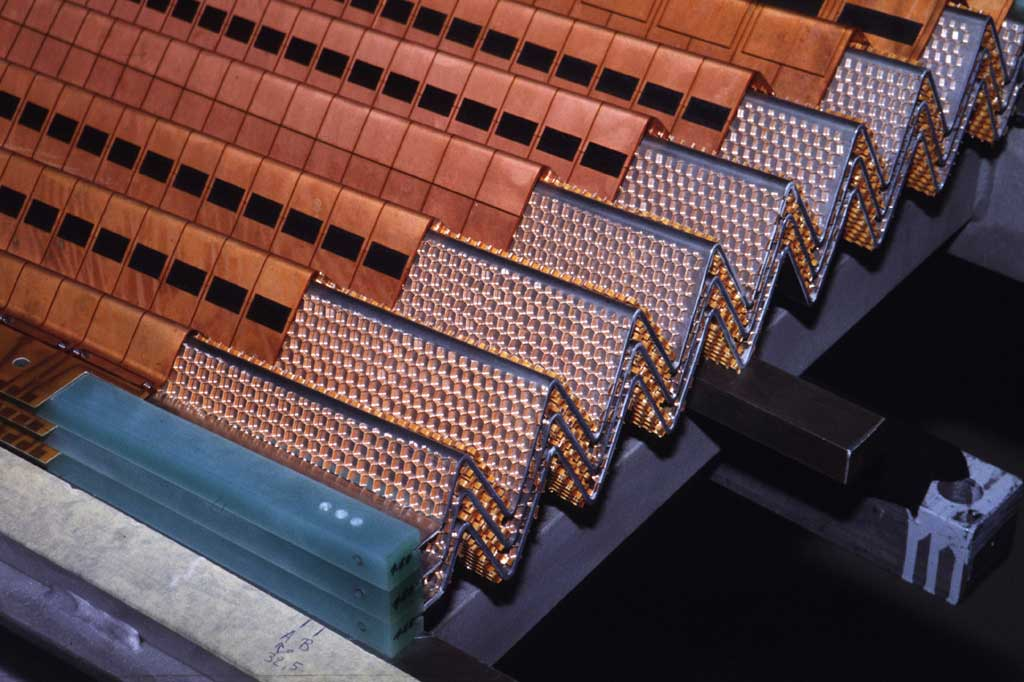
\includegraphics[width=\textwidth]{larpic}\makebox[0em][r]{\textcolor{natgreen}{\rule{\textwidth}{1pt}}}
    \end{center}
\end{minipage}
\begin{minipage}[b]{.4\textwidth}
    \begin{center}
    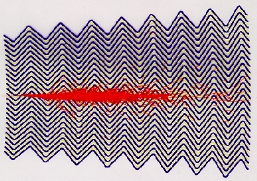
\includegraphics[width=\textwidth]{shower}\makebox[0em][r]{\textcolor{natgreen}{\rule{\textwidth}{1pt}}}
    \end{center}
\end{minipage}

\begin{minipage}[t]{.59\textwidth}
    \begin{center}
    \subcaption{A section of the LAr calorimeter.}
    \end{center}
\end{minipage}
~\begin{minipage}[t]{.4\textwidth}
    \begin{center}
    \subcaption{Illustration of a particle shower within the LAr calorimeter. \label{shower}}
    \end{center}
\end{minipage}

\begin{minipage}[b]{.59\textwidth}
    \begin{center}
    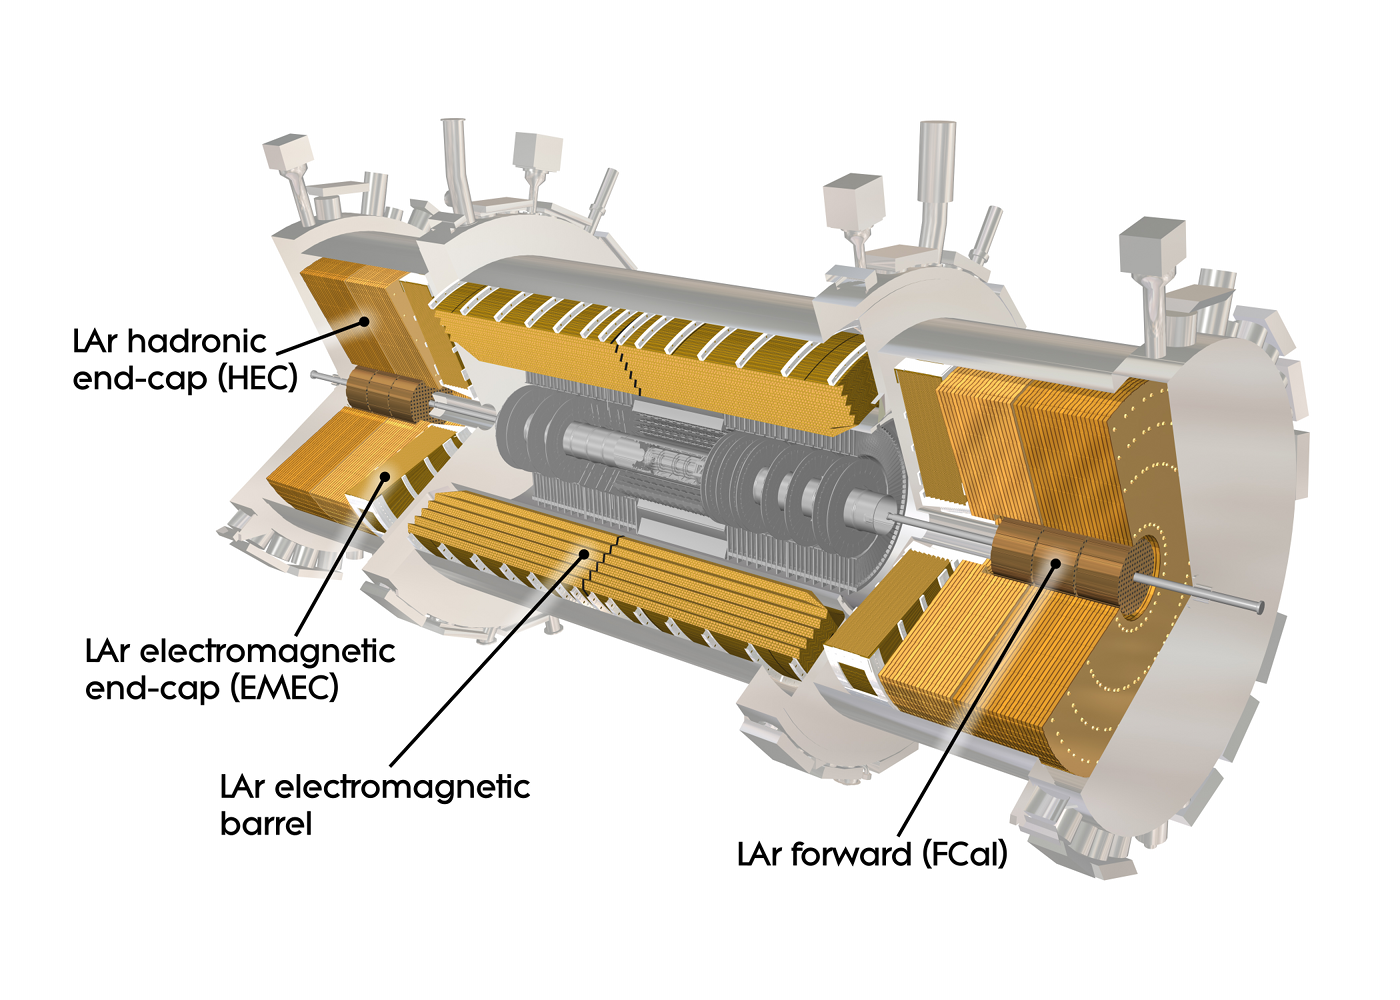
\includegraphics[width=1\textwidth]{figures/CaloDiag.png}
    \subcaption{Schematic showing the placement of the LAr calorimeters in \textsc{atlas}.}
    \end{center}
\end{minipage}
\begin{minipage}[b]{.4\textwidth}
\caption{Several figures \cite{atlasweb} that illustrate the design and functioning of the LAr calorimeters. These are sampling calorimeters, which have an absorbing medium (lead or steel) with layers of detecting medium (liquid argon) inserted regularly to keep track of the developing shower shape. In \textsc{atlas}, rather than having flat layers, the absorbing ans sensitive materials are interleaved in an accordion shape, visible in (a) and (b), which allows the detector electronics to be placed on the surface of the absorbing plates, rather than interrupting the calorimeter with non-sensitive signalling equipment.
\label{calostruc}}
\end{minipage}
\end{figure}

The iron and lead absorbing material in these calorimeters are constructed in an accordion shape, with liquid argon filling the gaps. The shape is visible in fig.~\ref{calostruc}. Plates carrying a high voltage are suspended in the middle of the space between accordion plates, which attract the ionised trail left by the passage of high energy charged particles, and detect the charge they deposit. The accordion shape allows readout electronics to run continuously out of the detector, rather than being interspersed as discreet layers in the absorbing material. This layout removes the need to interrupt the detector with non--sensitive communication channels.

For our purposes, the interesting quantities will be the energy deposited by photons and electrons. In the presence of matter, high--energy photons loose energy primarily through pair production, while electrons loose energy primarily through bremsstrahlung. The typical lengths travelled by both types of particle before undergoing such a process---their radiation lengths---depend on the material traversed, but are roughly equal to one another \cite{fernow:sampcal}. As illustrated in fig.~\ref{emshower}, both types of particles will undergo the same sort of evolution as they travel through an absorbing material, splitting into pairs of particles, each with a fraction of the energy of the parent particle, until the daughter particles fall below the energy where they can be absorbed by the material. This cascade of particles develops in a shower structure, as illustrated in fig.~\ref{shower}. Thus, we can measure the energy of the original particle both by how deep into the absorbing material it penetrates, or how many daughter particles it produces. \textsc{Atlas}' LAr calorimeters mainly use the second strategy.

\begin{figure}[htp]
\begin{minipage}[b]{.69\textwidth}
\begin{infilsf}\footnotesize
\begin{tikzpicture}[x=\textwidth*.95/3.5,y=\textwidth*.95/3.5]

\tikzset{photon/.style={decorate,decoration={snake,amplitude=1}},
         vert/.style={fill=black,circle,draw,inner sep=0pt,minimum size=2},
         grid/.style={draw=kugray!50}
         }
         
\draw[grid] (0,-.6) -- +(0,1.5) (1,-.6) -- +(0,1.5) (2,-.6) -- +(0,1.5) (3,-.6) -- +(0,1.5);
\draw (-.2,-.6) -- (0,-.6) node[below] {0} -- +(0,.05) +(0,0) -- ++(1,0) node[below] {1} -- +(0,.05) +(0,0) -- ++(1,0) node[below] {2} -- +(0,0.05) +(0,0) -- ++(1,0) node[below] {3} -- +(0,.05) +(0,0) -- ++(.3,0);
\draw (3.2,-.6) +(0,-1.1em) node[below left] {Depth in radiation lengths};

\draw (-.1,0) -- (0.4,0) node[vert] {} -- (1.7,-.2) node[vert] {} -- (2.7,-0.1) node[vert] {} -- (3.2,0) ;
\draw[photon] (0.4,0) -- (1.3,.2) node[vert] {};
\draw (1.3,.2) -- node[above] {\tiny$+$} (2.5,.5) node[vert] {} -- node[below] {\tiny$+$} (3.2,.4);
\draw[photon] (2.5,.5) -- (3.2,.7);
\draw (1.3,.2) -- (2.3,.1) node[vert] {} -- (3.2,.2);
\draw[photon] (2.3,.1) -- (3.2,.05) (2.7,-.1) -- (3.2,-.1) (1.7,-.2) -- (2.3,-.3);
\draw (3.2,-.3) -- (2.3,-.3) node[vert] {} -- node[below] {\tiny$+$} (3.2,-.5);



\end{tikzpicture}
\end{infilsf}
\end{minipage}\hfill
\begin{minipage}[b]{.3\textwidth}
\caption{A schematic description of an EM shower developing in an absorbing material. Here, a wavy line indicates a photon, a straight line indicates an electron, and a straight line with a `$+$' a positron. At each split, the two resulting particles carry away half the energy of the original particle. In a sampling calorimeter, a sensitive layer is typically inserted at intervals of one radiation length. \textsc{Atlas}' LAr calorimeters measure the magnitude of ionisation that is left in the liquid argon by the passage of the particle shower. Adapted from \cite{fernow:sampcal}.
\label{emshower}
}
\end{minipage}
\end{figure}

The shower can be initiated by material in the detector ahead of the calorimeter just as well as the material in the calorimeter. To account for this possibility, the first active layer, called the presampler, sits ahead of the first absorbing layer. Photons that undergo pair production sufficiently deep in the detector for the tracker to resolve at least one of the (anti--)electrons that are produced are treated as a separate object type, namely converted photons.

The calorimeter is divided into three layers, which are split into readout bins as illustrated in fig.~\ref{caldiv}. The first layer is very finely divided in the $\eta$ direction, and its readout cells will on occasion be referred to as `strips' in the `strip layer', as opposed to the `cells' in the other two layers. The energy deposited in the calorimeter is measured by the magnitude of the ionisation left in the active layers by the particle showers.

\begin{figure}[htp]
\begin{minipage}[b]{.69\textwidth}
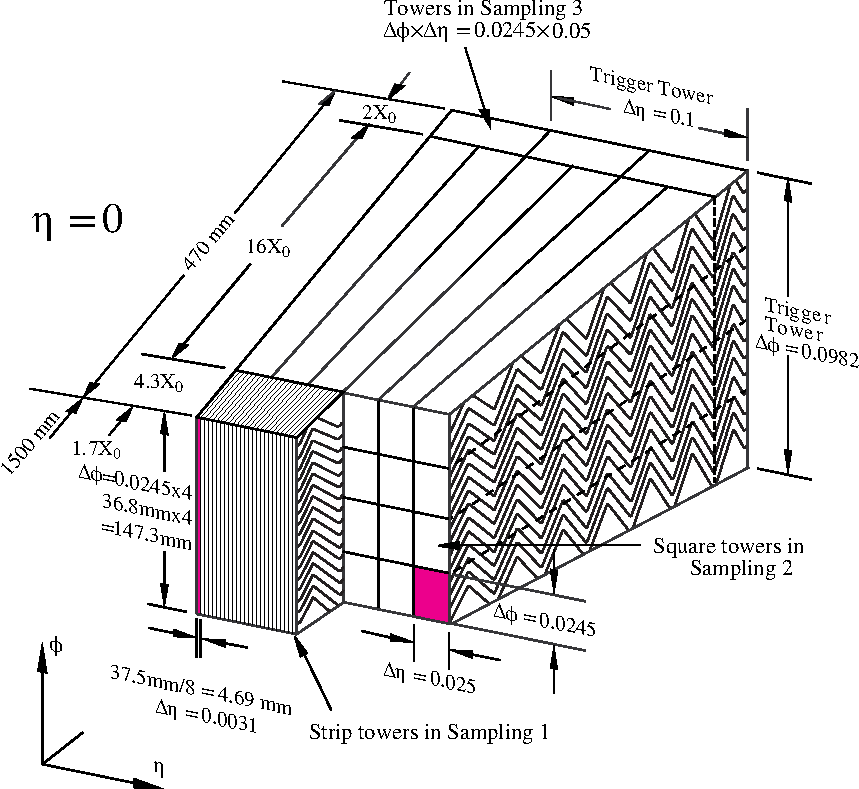
\includegraphics[width=\textwidth]{caldiv}
\end{minipage}
\begin{minipage}[b]{.3\textwidth}
\caption{The division of the EM calorimeter into detecting cells \cite{egede}. The first layer is divided into thin strips for the greatest resolution in the $\eta$ direction. The second layer is divided into roughly square cells, and comprises the bulk of the depth of the detector. The last layer is presumed to only be reached by the most energetic particles, and can have a coarser division without loosing resolution. This diagram is of the calorimeter at $\eta = 0$, closest to the interaction point. At higher $|\eta|$, the towers are angled so that they are still pointed toward the interaction point.
\label{caldiv}}
\end{minipage}
\end{figure}

The division of the calorimeter into layers gives us some resolution in depth when attempting to describe the shape of a shower. Showers initiated by different types of particles evolve in a slightly different way, which allows us discern the source of a shower by examining its shape. Additionally, with this shower shape information, we can extrapolate the direction from which a particle entered the calorimeter by looking at the shape of the shower, which is of particular importance when attempting to trace the origin of unconverted photons, which otherwise leave no trail in the detector.

\subsection{Photon identification}
The detector, then, provides information about clusters of energy deposits in the calorimeter and tracks reconstructed from hits in the tracking detector. Our task now is to identify those signals that have been left by photons.

We can build a set of candidates for deposits left by unconverted photons by taking those deposits in the calorimeter that do not have a track pointing to them. We expect converted photons to show up as pairs of electron tracks in the tracking detector that share a vertex away from the interaction point. However, we must account for the possibility that only one of the tracks are reconstructed, and so we also consider electrons tracks that only show hits in the straw detector as candidates for converted photons. These selection rules can then be written into a computer algorithm, which performs the event--by--event sorting for us \cite{phorec}. [hrrr]

This set will of course be contaminated with events that were not caused by photons: $\pi^0$ mesons also create calorimeter hits with no associated track, and QCD jets can mimic converted photons, among other possibilities. To attempt to sort genuine photon events from impostor events, we study the shape of the shower left in the calorimeter. To that end, we define the following shower shape variables \cite{Carminati}:

\begin{itemize}
\item $R_\text{had}$, the ratio of energy deposited in the hadronic calorimeter to the cluster energy in the EM calorimeter. Hadronic showers are expected to penetrate deeper into the hadronic calormieter than EM showers.
\item In the middle EM calorimeter layer, non-EM showers spread wider than electromagnetic ones. The variables that measure the shape of the shower in this layer are
\begin{itemize}
\item $R_\eta$, the ratio in $\eta$ of cell energies in 3 $\times$ 7 versus 7 $\times$ 7 cells.
\item $R_\phi$, the ratio in $\phi$ of cell energies in 3 $\times$ 7 versus 7 $\times$ 7 cells.
\item $w_{\eta 2}$, the width of the shower in the $\eta$ direction.
\end{itemize}
\item The strip layer, with its greater resolution in $\eta$, can pick out some of the internal structure of a jet. Hadron showers tend to show more than one maximum. Variables that measure the shape in the strip layer are
\begin{itemize}
\item $w_{s3}$, the shower width for three strips around the maximum strip.
\item $w_{s\text{ tot}}$, the total lateral shower width in the strip layer.
\item $F_\text{side}$, the faction of energy deposited outside a core of 3 central strips, but within 7 strips.
\item $\Delta E$, the difference in energy of the strip with the second largest energy deposited and the strip with the smallest energy deposited between the two leading strips.
\item $E_\text{ratio}$, the ratio of the energy difference associated with the
largest and second largest energy deposits, over the sum of these energies.
\end{itemize}
\end{itemize}

These variables form the selection criteria by which we declare a photon candidate to be an actual photon. The full list of variables above forms the tight selection criteria, while a shorter list, consisting of $R_\text{had}$, $R_\eta$ and $w_{\eta2}$ form the loose selection criteria. Separate cut values in these variables exist for different $\eta$ ranges. For a complete description, see \cite{Carminati}.

\subsection{Triggering and data collection}
While in full operation for the 2012, 8~TeV run, the LHC delivered a bunch crossing in \textsc{atlas}' interaction point every 50~ns. Reading out the whole detector produces 1.6~MB of information, which, if the detector were read out completely with every crossing, would produce a data rate of 34~TB/s.\footnote{For perspective, that is approximately equal to the estimated global IP traffic rate in 2015, according to \cite{wolframip}.} However, since only a fraction of these collisions produce interesting physics events, we can reduce the data rate to less prohibitive levels simply by not recording data from collision that do not produce interesting events. To accomplish this, we need a system that examines events in the detector as they occur, and trigger recording whenever it sees an interesting event. In \textsc{atlas}, this trigger system has three levels, which are described in detail in \cite{detectorpaper}. 

The level--1 trigger examines events in real time as they occur in the detector. To do so, the trigger logic is run on specialised hardware built in to the detectors. As a result, each trigger only has access to information from the detector its hardware is attached to. Chalorimeter triggers, for example, do not have access to information from the tracking system at the first trigger level. Also, computationally intensive tasks, such as track reconstruction, can not be completed in the window of time available to the level--1 trigger, and so are also not available. The next trigger level, level--2, is run on the full set of information from an event, on those events which pass the level--1 filter. The final trigger level works with fully reconstructed events and derived physical observables. This requres more time and processing power than is available at the previous levels, but it also identifies interesting events with the same quality of information as will be used in the subsequent analysis. All three triggers in combination cuts the final event rate to 300 events per second, with a peak rate of 600 events.

For this thesis, we shall use data taken during the 8~TeV run in 2012. The amount of data taken at any given time depends on the conditions of the beam, which can be summarised in the instantaneous luminosity, and the conditions of the detector, which may only capture a fraction of the events produced at any given time. Figure~\ref{intlumi} gives the distribution of integrated and captured luminosity over the course of the year.

\begin{figure}[htp]
\begin{minipage}[b]{.69\textwidth}
\hspace{-1em}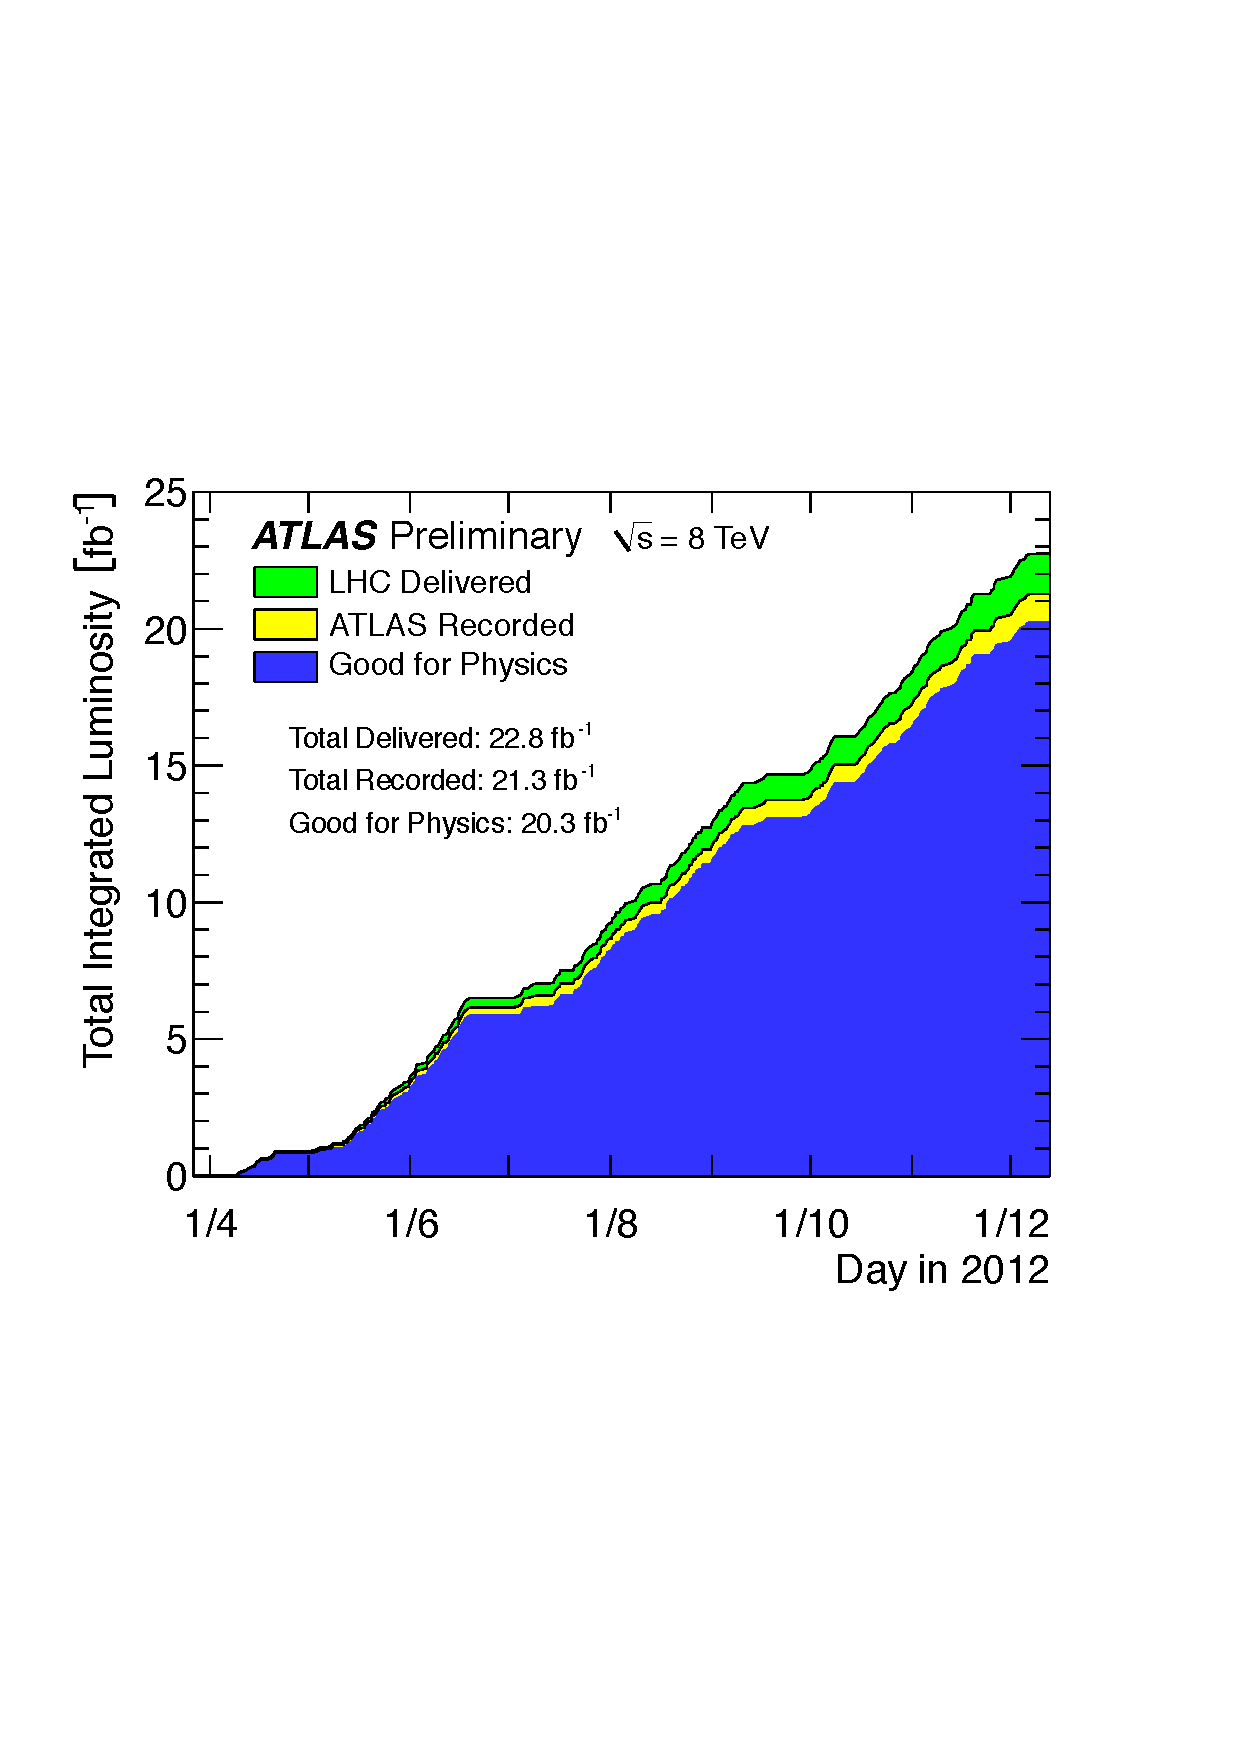
\includegraphics[width=\textwidth]{figures/intlumi}
\end{minipage}\hfill\begin{minipage}[b]{.3\textwidth}
\caption{A plot showing the integrated luminosity delivered by the LHC (green), recorded by ATLAS (yellow), and fulfilling data quality criteria (blue), over the course of the 8 TeV run in 2012 \cite{publiclumi}.
\label{intlumi}}
\end{minipage}
\end{figure}

Unfortunately, the triggers that are implemented in \atlas{} do not guarantee that the event rate remains within the technical limitations of the readout system. To stay within those limits, \atlas{} prescales certian triggers, when they originate from a trigger that produces more events than it is considered worth keeping,\footnote{Explaining how it is decided whether data is worth keeping would veer into a discussion of \atlas{} internal politics, which is a topic beyond the scope of this thesis.} which means simply that a fraction of event that pass a trigger are not recorded. The diphoton channel is important to the search for the Higgs boson, however, so the triggers that produce diphotons events have not been prescaled.
